El modelo estándar caliente del Big Bang teoriza que las condiciones iniciales para el Universo sean dadas por campo gaussiano casi invariante o espectro de \matterspectrum ~ \citep{rubakov_harrison--zeldovich_2009}, predicción del modelo de inflación cósmica. Por lo que si se considera el estado inicial del Universo aleatorio bajo ciertas consideraciones, entonces, los postulados sobre las inhomogeneidades en el Universo necesitan ser estadísticas por naturaleza. 

En la actualidad la radiación del fondo cósmico de microondas (\CMB, de sus siglas en inglés \textbf{C}osmic \textbf{M}icrowave \textbf{B}ackground) descubierto a mediados de los años 1960 y el corrimiento al rojo cosmológico son conjuntamente evidencia experimental disponible para válidar aspectos importantes de la teoría del Big Bang. Se teoriza que unos 379 000 años después del Big Bang (per\'iodo de la última dispersión) la temperatura del Universo era de unos $3000~K$, la misma ha caído en un factor de aproximadamente $1100~K$ debido a la expansión del Universo. Según se expande el Universo, los fotones del fondo cósmico de microondas se desplazan hacia el rojo, haciendo que la temperatura de radiación sea inversamente proporcional al factor de escala del Universo.

La radiación~\CMB~parece a primera vista isótropa, posee pequeñas variaciones en la temperatura predichas por el modelo de Big Bang, estas peque\~nas anisotropías o inhomogeneidades teorizadas fueron detectadas finalmente en los años 90 por el satélite de la NASA \textbf{COBE} (\textbf{C}osmic \textbf{B}ackground \textbf{E}xplorer) entre 1989 y 1996, considerandose variaciones de densidad del universo primitivo y su descubrimiento arroja indicios de la formación de las primeras estructuras de gran escala y la distribución de galaxias del universo actual. 

En el 2001 la agencia espacial americana NASA lanza el~\WMAP~( de sus siglas en inglés \textbf{W}ilkinson \textbf{M}icrowave \textbf{A}nisotropy \textbf{P}robe) satélite capaz de estudiar con gran detalle la radiación~\CMB~consiguiendo el mapa más completo posible por la humanidad. Otros instrumentos han detectado aún con más detalle y a mayor resolución angular las anisotropías del \CMB, como el Cosmic Background Imager pero en sólo unas zonas del cielo. %Los datos aportados por el \textbf{\WMAP} revelan un universo en expansión formado por un 4\% de materia bariónica, un 22 \% de materia oscura y un 74 \% de energía oscura. 
El 2009 la Agencia Espacial Europea lanzó el Planck, un satélite de capacidades mucho mayores todavía que el \WMAP.

La anisotropía del fondo de radiación de microondas está dividida en dos tipos: anisotropía primaria (debida a efectos que ocurren en la última superficie de dispersión y en la anterior) y la anisotropía secundaria (debida a efectos, como las interacciones con gases calientes o potenciales gravitacionales, entre la última superficie de dispersión y el observador.



%La Sonda de Anisotropía de Microondas Wilkinson (WMAP, de sus siglas en ingles \textbf{W}ilkinson \textbf{M}icrowave \textbf{A}nisotropy \textbf{P}robe) fue una misión del Explorador de la \textbf{NASA} lanzado en 2001 para realizar mediciones fundamentales de la cosmología, el estudio de las propiedades de nuestro universo en su conjunto.

La imagen detallada de la temperatura de la radiación de fondo cósmico de microondas (\CMB, de sus siglas en inglés \textbf{C}osmic \textbf{M}icrowave \textbf{B}ackground) de todo el cielo del universo fue recreada a partir diversos intento de medición y con la red de datos del~\WMAP, esta revela fluctuaciones de temperatura de 13.77 mil millones de años (mostradas como diferencias de color) que corresponden a las semillas que crecieron para convertirse en galaxias. La señal de nuestra galaxia se resta con los datos de múltiples frecuencias, la resultante (Fig. \ref{universo}a) muestra un rango de temperatura de $\pm~200~\mu K$.

\begin{figure}
\centering
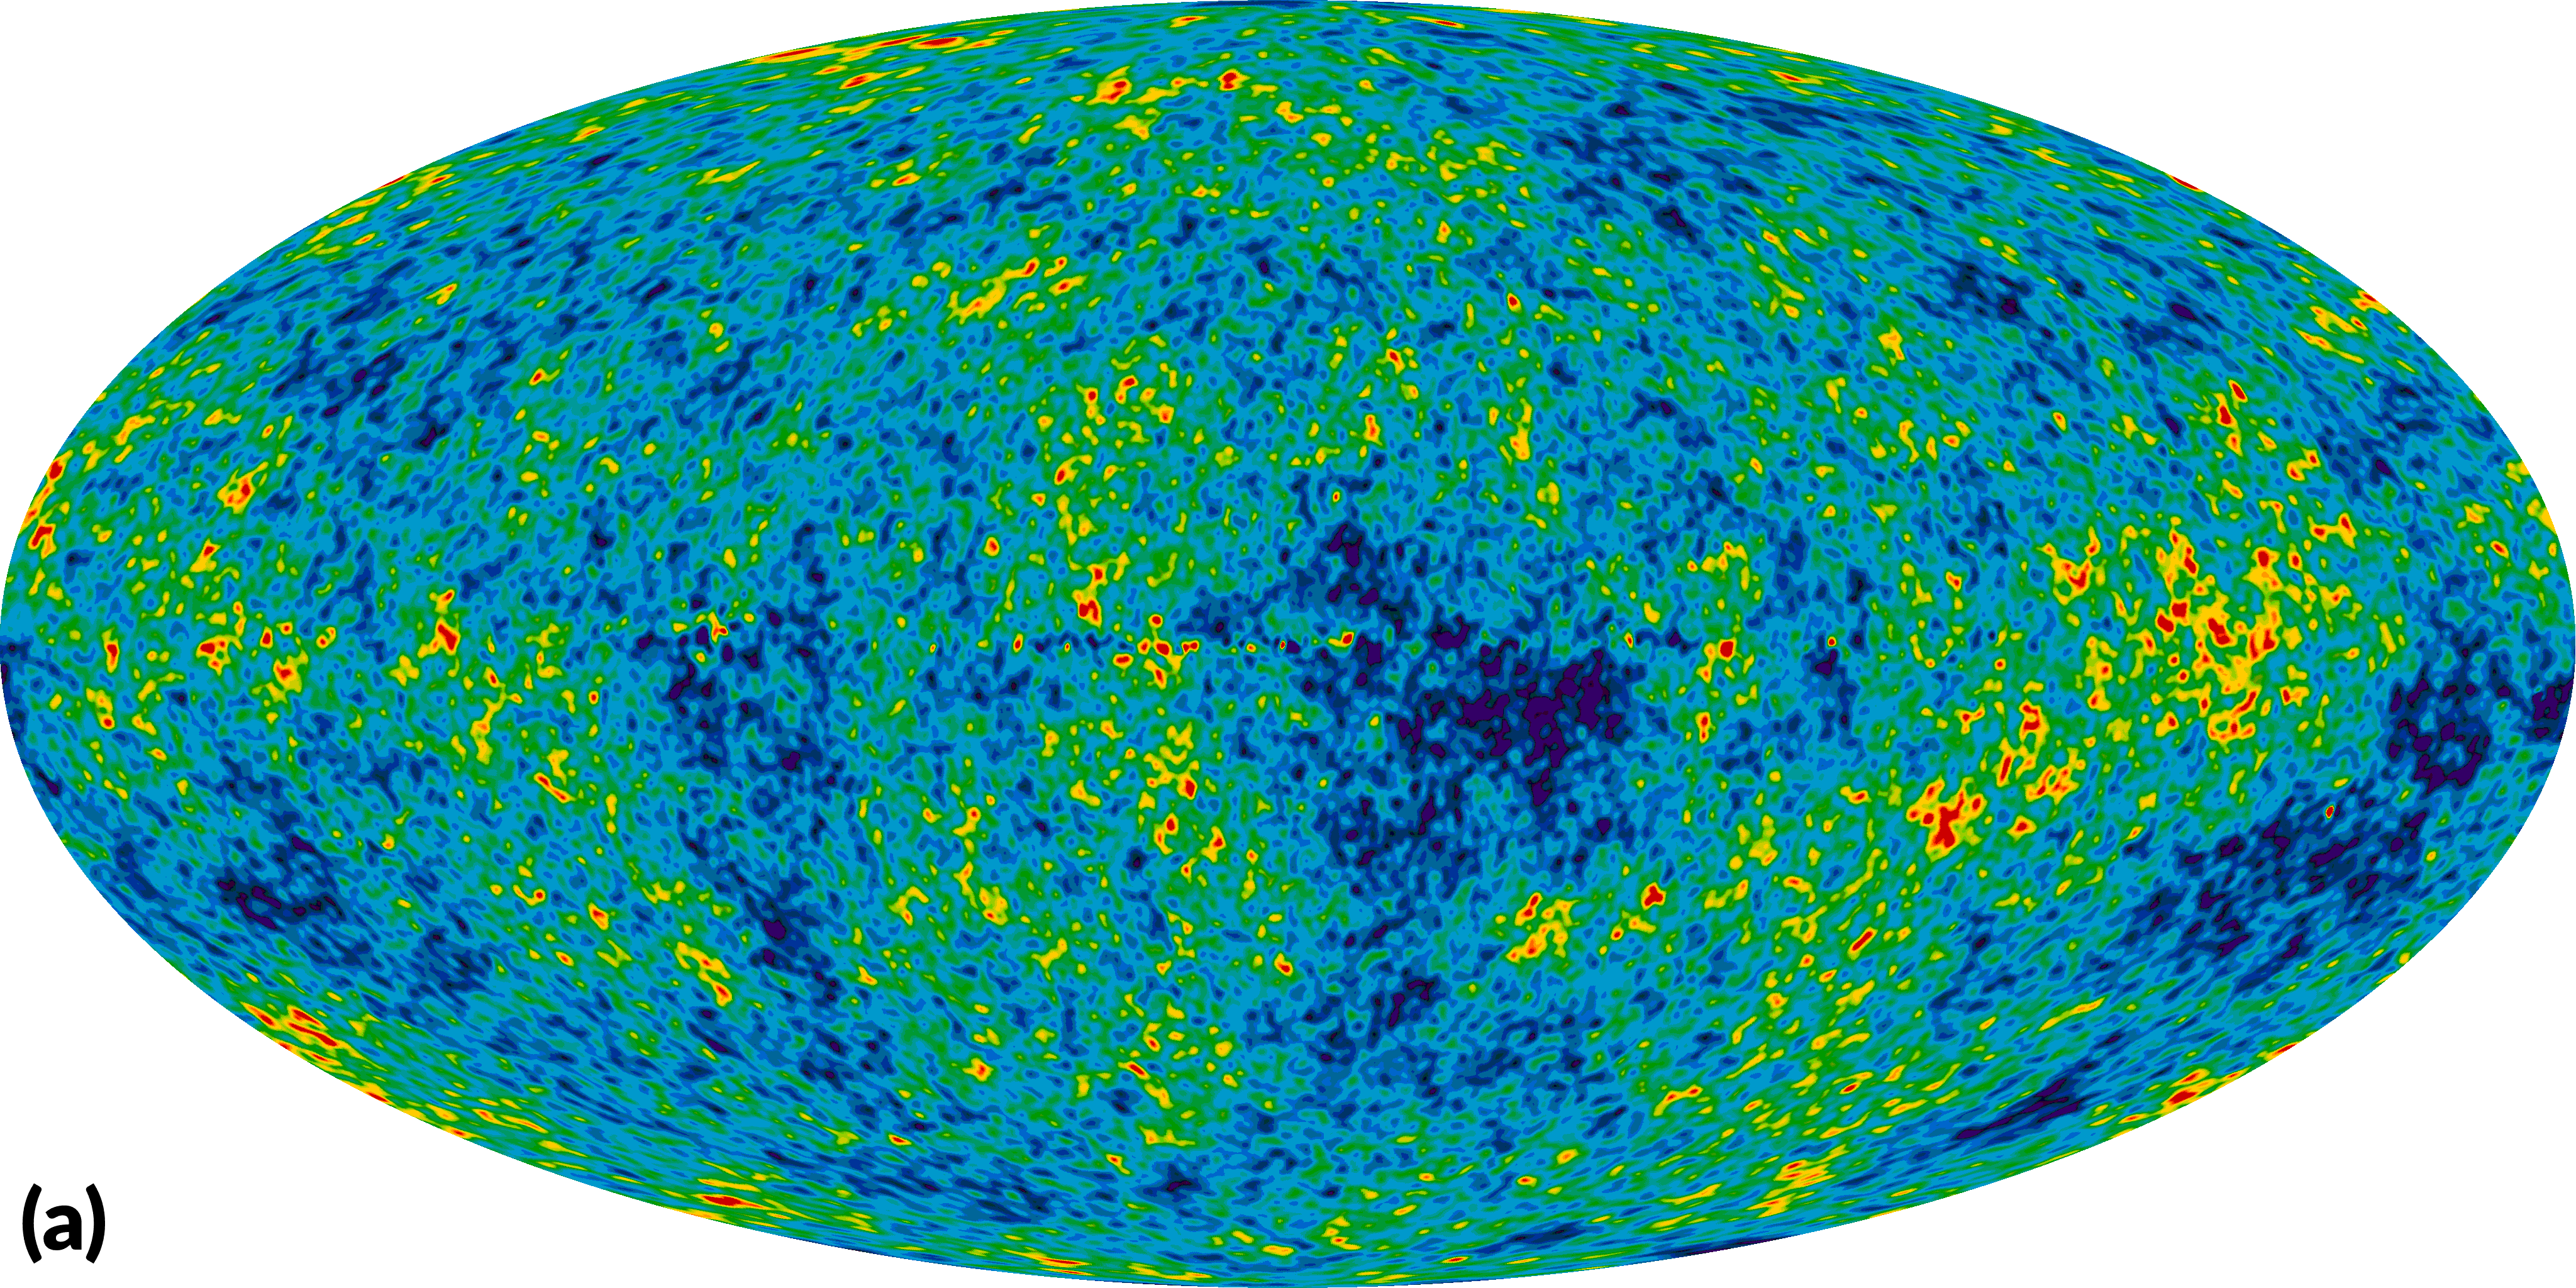
\includegraphics[width=0.49\textwidth]{Fisica_de_Particulas/imagenes/universo.png}
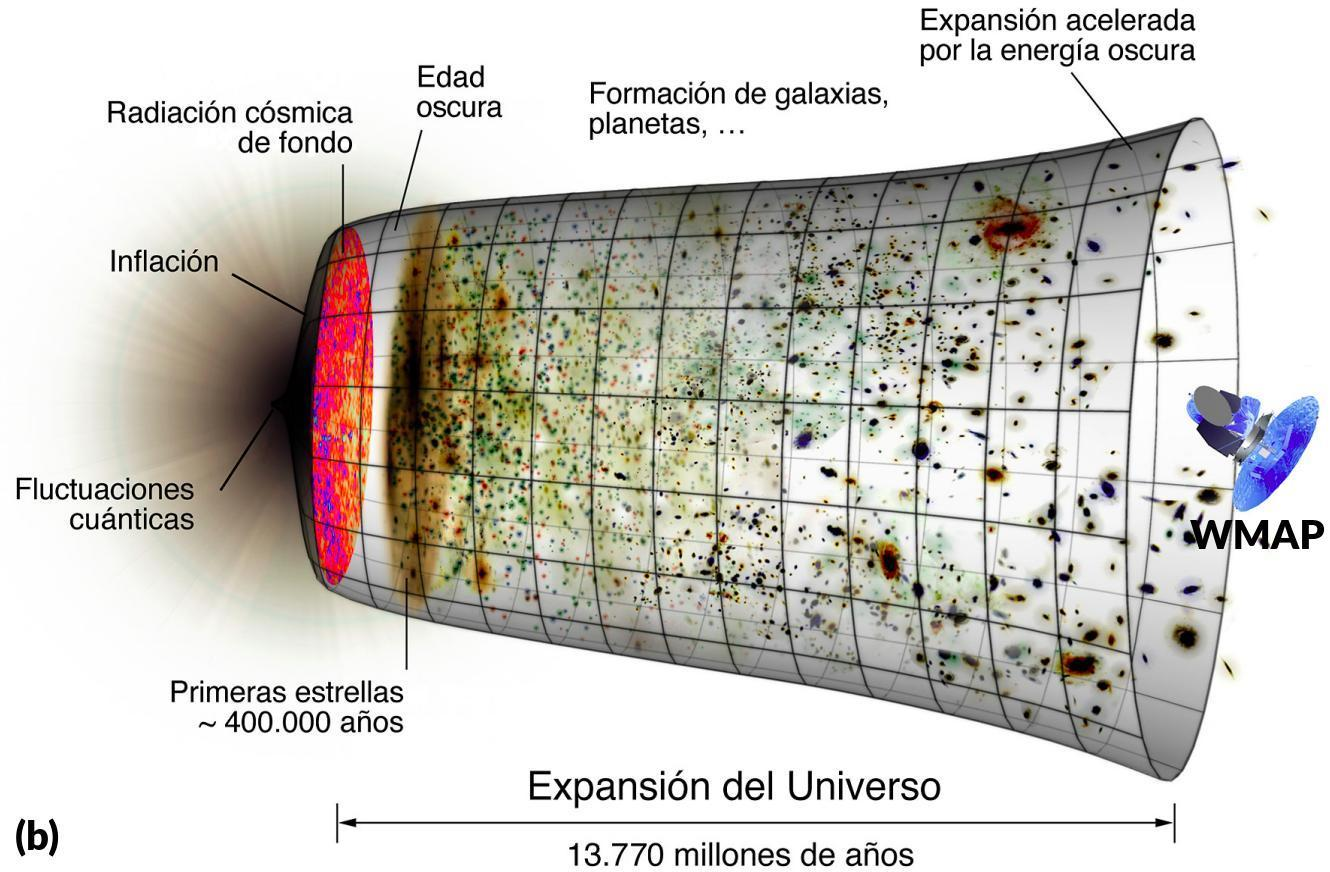
\includegraphics[width=0.49\textwidth]{Fisica_de_Particulas/imagenes/Universo_evo0.jpg}
\caption{(a) Mapa de anisotropías de temperatura de~\CMB~según lo observado por el telescopio ~\WMAP. Página de origen: \url{https://wmap.gsfc.nasa.gov/media/121238/index.html}; (b) Representación de la evolución del universo a lo largo de 13.77 mil millones de a\~nos. Página de origen: \url{https://wmap.gsfc.nasa.gov/media/060915/index.html}}
\label{universo}
\end{figure}

En el modelo de concordancia, a épocas muy tempranas del Universo, todas
las especies ya mencionadas estuvieron térmicamente acopladas en el gas primigenio. Conforme el Universo se expande, su temperatura disminuye y las diversas especies se desacoplan del gas, dando lugar a épocas con propiedades muy particulares (Fig. \ref{universo2}) las cuales a grandes rasgos son:
\begin{itemize}
\item[-] \textbf{[}$\mathbf{0s ~ - ~ t_p \approx 5.3(9)\cdot 10^{-44}}$\textbf{s] Época de Planck :} es el período de tiempo en la historia en segundos, es el universo más temprano durante el cual las cuatro fuerzas fundamentales (interacción nuclear fuerte, interacción nuclear débil, interacción electromagnética e interacción gravitatoria) están unificadas y no existen todavía las partículas elementales, la mecánica cuántica estándar teoriza que el tiempo de plack está dado por:
\begin{equation}
t_p ~ \equiv ~ \sqrt{\hbar G/c^5}
\end{equation}
donde $G$ es la constante de Gravitación Universal, $c$ es la constante de gravitación universal, $\hbar$  es la constante de Planck reducida. $t_p$ tiempo de Planck o cronón, es la unidad de tiempo, considerada como el intervalo temporal que representa el instante de tiempo más pequeño en el que las leyes de la física podrían ser utilizadas para estudiar la naturaleza y evolución del Universo.
%% articulo http://laenciclopediagalactica.info/2019/04/02/origen-y-evolucion-del-universo-temprano/
%% http://pelusa.fis.cinvestav.mx/tmatos/CV/3_RecursosH/Dr/Juan_Aldebaran.pdf
%% http://laenciclopediagalactica.info/2019/04/02/origen-y-evolucion-del-universo-temprano/
\item[-] \textbf{[}$(\mathbf{t_p ~ - ~ 10^{-5}s)}$ \textbf{ ]Época de Gran Unificación :}  asumiendo que la naturaleza está descrita por una Teoría de Gran Unificación, este es el período en la evolución del universo temprano que siguió a la Época de Planck. La temperatura durante esta época se teoriza en 1027 K con una energía de $1015 ~GeV ~ \gtrsim ~10 ~ TeV$. Así que, todos los procesos (y las hipótesis para explicarlos) que ocurren en esta fase del Universo tales como el inicio de la gran explosión, inflación, bariogénesis y otros, son especulativos.
\begin{itemize}
\item \textbf{[}$(\mathbf{t_p ~ - 10^{-35}s )}$\textbf{] Primera congelación :}  la gravedad se separó para siempre de las otras fuerzas, y la expansión universal se opuso por primera vez a la gravedad. Antes de ese tiempo se le conoce como el período inflacionario.
\item \textbf{[}$(\mathbf{10^{-35}s ~ - ~ 10^{-10}s)}$\textbf{] Segunda congelación :}  se congela la fuerza fuerte, permitiendo la creación de los átomos.
\item \textbf{[}$(\mathbf{10^{-10} - 10^{-5}s )}$\textbf{] Tercera congelación :} se congela la fuerza débil y la fuerza electromagnética.
\end{itemize}

\item[-] \textbf{[}$(\mathbf{10^{-5}s - 1s )}$\textbf{] Universo temprano :} la energía decae a $200 ~ MeV$ permitiendo la transición de fase quark-gluón(confinamiento en bariones y mesones), existe un plasma caliente con todos los compuestos existentes en equilibrio térmico, con la expanción la temperatura, energía y por lo tanto la tasa de interacción disminuyen, desacoplando el plasma. Cuando la energía del Universo alcanza $\thicksim 0.5 ~ MeV$, solamente los electrones, protones, neutrones y los fotones permanecen acoplados en el plasma, mientras el resto de las especies, como los neutrinos ($\backsim 1 ~ MeV$), ya se han desacoplado.

\item[-] \textbf{[}$(\mathbf{ 1s ~ - ~ 3/5 ~ min )}$\textbf{] Nucleosíntesis :} Momento en que la energía del Universo alcanza $\thicksim ~0.05 ~ MeV$ las reacciones nucleares llegan a ser eficientes por lo tanto, los protones y neutrones libres forman elementos ligeros como el helio, litio, deuterio. Las predicciones teóricas de la nucleosíntesis primigenia ajustan bastante bien los datos observacionales concluyendo que la densidad bariónica en el Universo es $\backsim ~0.05$ de la densidad crítica fundamentando
así que la presencia de materia no bariónica en el Universo.

\item[-] \textbf{[}$\mathbf{6~ \cdot ~ 10^{5}}$ \textbf{a\~nos] Igualdad materia-radiación :} la energía del Universo es $\thicksim 1 ~ eV$ y la densidad de materia es igual a la densidad de radiación $\Omega_x(t) = \Omega_z(t)$, anteriormente había un dominio de la radiación, deapués de está época hay una prevalencia de la materia, las observaciones del \CMB ~ en el corrimiento del rojo $z = 3100$ fundamentan este hecho.

\item[-] \textbf{[} $\mathbf{37.5 ~ \cdot ~ 10^{5}}$ \textbf{a\~nos] Recombinacion :} la energía del Universo disminuye a $\thicksim ~0.1 eV$, los fotones y los electrones se desacoplan de la materia como resultado de la dispersión de Compton, como resultando hay una recombinación de los electrones libres con los protones, con la formación de átomos los fotones puedan viajar en el Universo como reliquias térmicas sin ser dispersados por los electrones y que hoy podemos observar como \CMB ~ en el corrimiento del rojo corrimiento $z \approx 1090$.

\item[-] \textbf{[}$\mathbf{1.377 ~ \cdot ~ 10^{10}}$ \textbf{a\~nos] Formación de estructuras} Las peque\~nas perturbaciones en la distribución de la materia oscura comienzan a crecer debido a la acción de la fuerza de gravedad dando lugar a la formación de grandes estructuras en el Universo. Los pozos gravitacionales de estas estructuras gravitacionales atraen a su vez a la materia bariónica dando a lugar a las galaxias y cúmulos de galaxias.
\end{itemize}

\begin{figure}[t!]
\centering
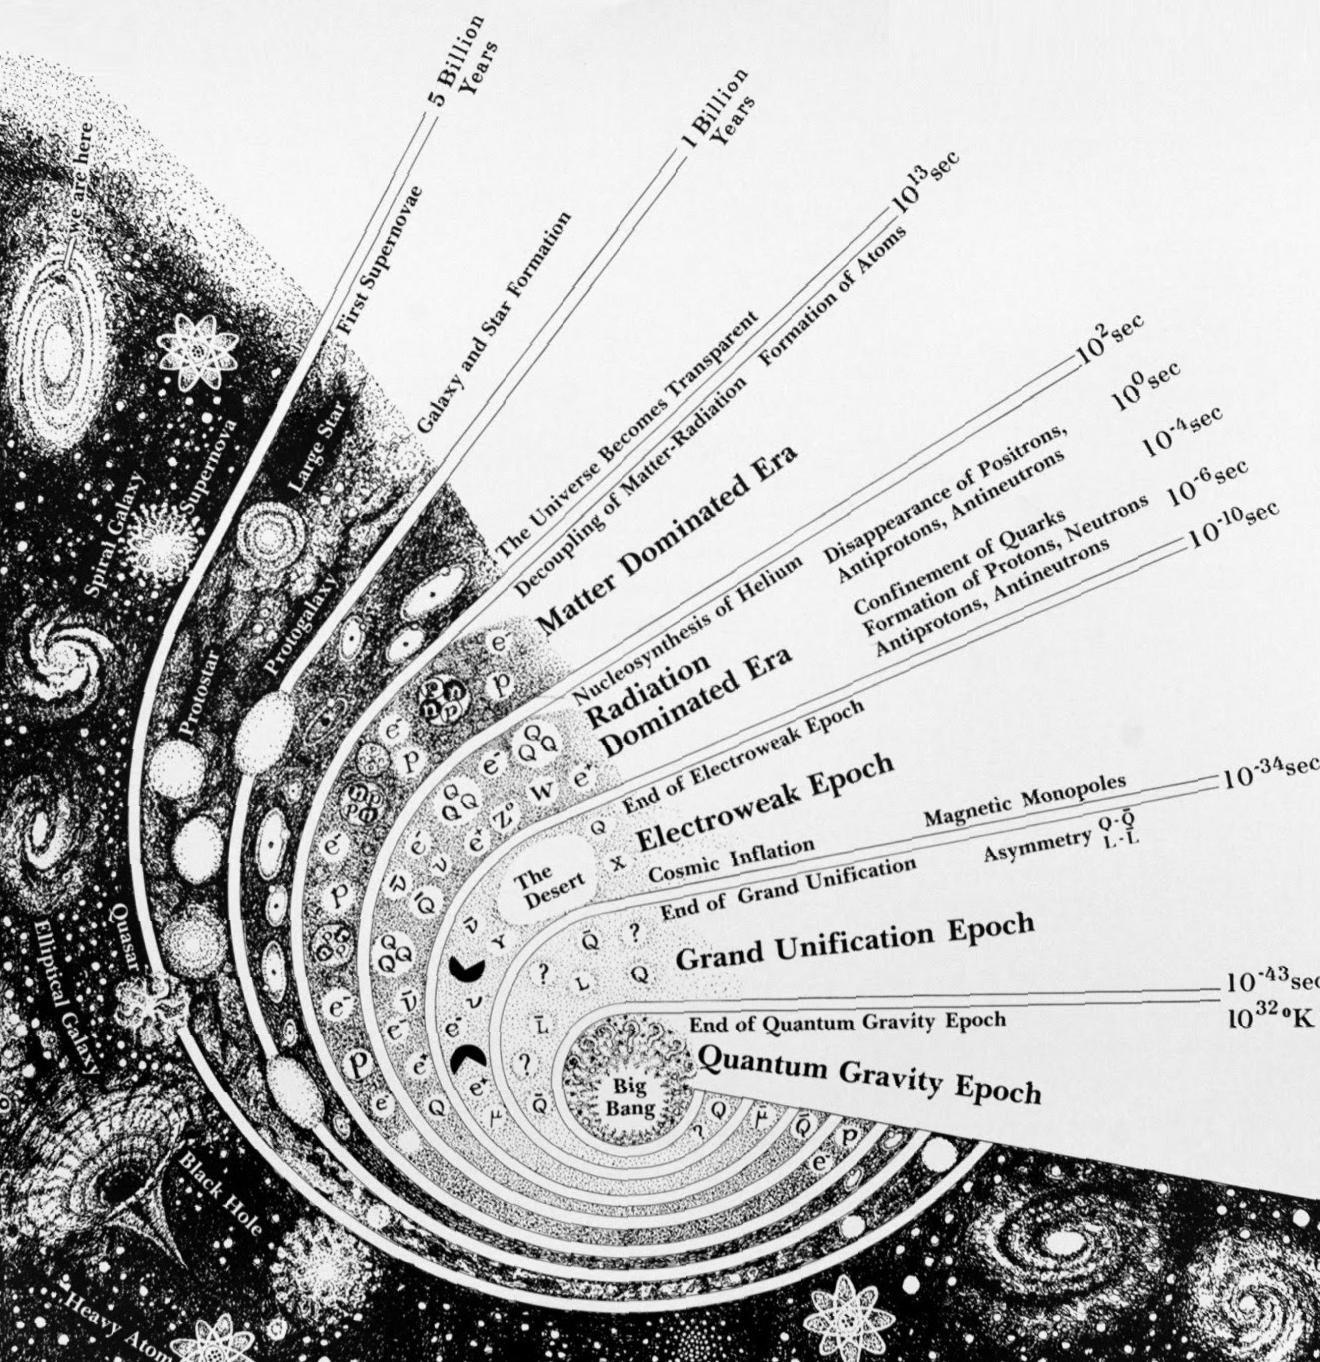
\includegraphics[width=0.6\textwidth]{Fisica_de_Particulas/imagenes/History_of_the_Universe_(Fermilab_1989).jpg}
\caption{La historia del Universo. Página de origen: \url{https://notodoeskippel.blogspot.com/2014/03/el-segundo-primordial.html}}
\label{universo2}
\end{figure}

El extremo izquierdo  de la Fig. \ref{universo}b representa el momento más temprano que ahora podemos investigar, cuando un período de ``inflación'' produjo una explosión de crecimiento exponencial en el universo. (El tamaño se representa por la extensión vertical de la cuadrícula en este gráfico). Durante los próximos miles de millones de años, la expansión del universo se desaceleró gradualmente a medida que la materia en el universo se empujó sobre sí misma a través de la gravedad. Más recientemente, la expansión ha comenzado a acelerarse nuevamente a medida que los efectos repulsivos de la energía oscura han llegado a dominar la expansión del universo. La luz incandescente vista por ~ \WMAP ~ se emitió aproximadamente 375.000 a\~nos después de la inflación y ha atravesado el universo en gran medida sin impedimentos desde entonces. %Las condiciones de tiempos anteriores están impresas en esta luz; También forma una luz de fondo para desarrollos posteriores del universo.
Al analizar detenidamente el espectro de potencia, los cosmólogos determinaron que nuestro universo es espacialmente plano con un 0,5\% de margen de error.

El satélite artificial Planck como parte del programa científico Horizon 2000 de la Agencia Espacial Europea es lanzado en el 2009 con la intención de detectar las anisotropías en el fondo cósmico de microondas en casi todo el cielo menos un octavo, con una resolución y sensibilidad sin precedentes. 

La información obtenida por el satélite Planck del ~\CMB~ muestra pequeñas fluctuaciones de temperatura que corresponden a regiones de densidades ligeramente diferentes en épocas muy tempranas, que representan las semillas de toda estructura futura resultado de las fluctuaciones que surgieron inmediatamente después del Big Bang y que se extendieron durante el período de expansión acelerada (inflación). Diseñado para mapear estas fluctuaciones en todo el cielo con mayor resolución y sensibilidad que nunca pudiendo determinar la composición y la evolución del Universo desde su nacimiento hasta nuestros días \citep{planck_collaboration_planck_2019}.

En general, la información extraída del nuevo mapa de Planck proporciona una excelente confirmación del modelo estándar de cosmología con una precisión sin precedentes, estableciendo un nuevo punto de referencia en nuestro manifiesto de los contenidos del Universo y debido a que la precisión del mapa de Planck es tan alta, también permitió revelar algunas características peculiares inexplicables que pueden requerir una nueva física para ser entendidas.

Entre los hallazgos más sorprendentes están:
\begin{itemize}
\item[-] Las fluctuaciones en las temperaturas de ~ \CMB ~ a grandes escalas angulares no coinciden con las predichas por el modelo estándar; sus señales no son tan fuertes como se esperaba de la estructura a menor escala revelada por Planck.
\item[-] Se reafirma la asimetría en las temperaturas medias en hemisferios opuestos del cielo. Esto va en contra de la predicción hecha por el modelo estándar de que el Universo debería ser ampliamente similar en cualquier dirección que miremos.
\item[-] Se reafirma la existencia de un punto frío se extiende sobre un parche de cielo que es mucho más grande de lo esperado.
\end{itemize}
Estos último dos puntos ya se habían intuido con la misión ~ \WMAP ~ de la NASA, pero fueron ignorados en gran medida debido a las dudas persistentes sobre su origen cósmico \citep{planck_collaboration_planck_2019}.

Una forma de explicar las anomalías es proponer que el Universo, de hecho, no es el mismo en todas las direcciones en una escala mayor de lo que podemos observar. En este escenario, los rayos de luz del CMB pueden haber tomado una ruta más complicada a través del Universo de lo que se entendía anteriormente, lo que resulta en algunos de los patrones inusuales observados hoy, sin embargo, sin la consideración de las anomalías, los datos de Planck se ajustan espectacularmente bien a las expectativas de un modelo bastante simple del Universo.

Esto permitió obtener valores mas refinados de los obtenidos por el ~ \WMAP ~ de la composición de la materia que compone el universo, sus resultados fueros 4.9\% de la masa bariónica. La materia oscura, que hasta ahora solo se ha detectado indirectamente por su influencia gravitacional, representa el 26.8\% y la energía oscura con un porciento de 68.3\% siento la fuerza misteriosa posible responsable de acelerar la expansión del Universo.

Los datos de Planck establecen la velocidad a la que el Universo se está expandiendo hoy(constante de Hubble) con $H_0 = 67.15~km~s^{-1} ~Mpc^{-1}$ implicando que la edad del Universo teorizada en la Fig. \ref{universo}b. 

%Según el Principio cosmológico debemos pensar que cualquier punto del universo es un buen punto para ser considerado como un supuesto ``centro'', pues desde cualquier punto tendremos las mismas observaciones en cuanto a expansión del universo y densidad, esta idea es necesaria para obtener el valor de la densidad crítica ($\rho_c$) que es la densidad de la materia en el universo necesaria para detener la expansión del mismo en un tiempo infinito, con valor de $\rho_c = 1.88~h 2 \times 10−26 kg/m^3$ implementando \href{https://es.wikipedia.org/wiki/Ecuaciones_de_Friedmann}{las ecuaciones de Friedmann} (ver referencia \cite{vazquez-gonzalez_materia_2008}) %https://www.astrobitacora.com/que-forma-tiene-el-universo/?utm_content=bufferd33ed&utm_medium=social&utm_source=pinterest.com&utm_campaign=buffer


%la densidad de masa promedio del Universo en unidades de la llamada densidad cr´ıtica 


%\begin{figure}[h]
%\centering
%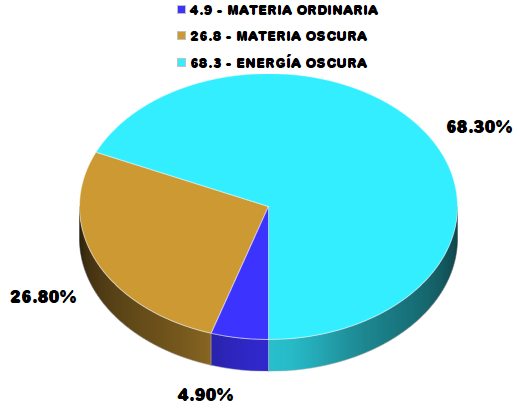
\includegraphics[width=0.49\textwidth]{Fisica_de_Particulas/imagenes/composicion0.png}
%\caption{Composición de la materia en el universo. Página de origen: %
%\url{https://wmap.gsfc.nasa.gov/media/121236/index.html}}
%\label{universo}
%\end{figure}





